% Opsætter KU Tex dokument
%%%%%%%%%%%%%%%%%%%%%%%%%%%%%%%%%%%%%%%%%%%%%%%%%%%%%%%%%%%%%%%%%%%%%%%%%%%%%%%%
\documentclass{article}                                                        %
\usepackage[a4paper, hmargin={2.8cm, 2.8cm}, vmargin={2.5cm, 2.5cm}]{geometry} %
\usepackage{eso-pic}  % \AddToShipoutPicture                                   %
\usepackage{graphicx} % \includegraphics                                       %
\usepackage{subfig}    
\usepackage{setspace}                                                        %
%%%%%%%%%%%%%%%%%%%%%%%%%%%%%%%%%%%%%%%%%%%%%%%%%%%%%%%%%%%%%%%%%%%%%%%%%%%%%%%%

% Pakker til skrifttyper, tekst osv.
%%%%%%%%%%%%%%%%%%%%%%%%%%%%%%%%%%%%%%%%%%%%%%%%%%%%%%%%%%%%%%%%%%%%%%%%%%%%%%%%
    \usepackage[utf8]{inputenc}  % Implementere Unicode                        %
    \usepackage[T1]{fontenc}     % Unicode skrifttype fx. é skrives som 1 tegn %
    \usepackage[english]{babel}   % Dansk Ordbog                                %
    \usepackage{microtype}       % Forbedre linjeombrydningen                  %
    \usepackage{libertine}       % Skrifttype                                  %
%%%%%%%%%%%%%%%%%%%%%%%%%%%%%%%%%%%%%%%%%%%%%%%%%%%%%%%%%%%%%%%%%%%%%%%%%%%%%%%%

% Pakker til matematik og kode.
%%%%%%%%%%%%%%%%%%%%%%%%%%%%%%%%%%%%%%%%%%%%%%%%%%%%%%%%%%%%%%%%%%%%%%%%%%%%%%%%
    \usepackage{mathtools}       % Udvidelse til amsmath pakken                %
    \usepackage{amsthm}          % Pakke til bevisførelse                      %
    \usepackage{amssymb}         % Extra matematiske symboler                  %				
	\usepackage{mychemistry}												   %
	\usepackage[version=3]{mhchem}											   %
	\usepackage{wrapfig}													   %
	\usepackage{siunitx}	
	\usepackage{anyfontsize}
	\usepackage{url}
	\usepackage{ragged2e}
	\usepackage{algorithm2e}
	\usepackage[final]{pdfpages}
	\usepackage{listings}

	\definecolor{light-gray}{gray}{0.85}
	\definecolor{dkgreen}{RGB}{0.0,128.0,43.0}
	\lstdefinelanguage{FSharp}%
{morekeywords={let, new, match, with, rec, open, module, namespace, type, of, member, % 
and, for, while, true, false, in, do, begin, end, fun, function, return, yield, try, %
mutable, if, then, else, cloud, async, static, use, abstract, interface, inherit, finally, int },
  otherkeywords={ let!, return!, do!, yield!, use!, var, from, select, where, order, by },
  keywordstyle=\color{bluekeywords},
  sensitive=true,
  basicstyle=\ttfamily,
	breaklines=true,
  xleftmargin=\parindent,
  aboveskip=\bigskipamount,
	tabsize=4,
  morecomment=[l][\color{dkgreen}]{///},
  morecomment=[l][\color{dkgreen}]{//},
  morecomment=[s][\color{dkgreen}]{{(*}{*)}},
  morestring=[b]",
  showstringspaces=false,
  literate={`}{\`}1,
  stringstyle=\color{redstrings},
}
	
	\lstset{frame=tb,
  	language=FSharp,			%CHANGE LANGUAGE
  	aboveskip=3mm,
  	belowskip=3mm,
  	showstringspaces=false,
  	columns=flexible,
  	basicstyle={\small\ttfamily},
  	numbers=none,
  	numberstyle=\tiny\color{gray},
  	keywordstyle=\color{blue},
  	commentstyle=\color{dkgreen},
  	stringstyle=\color{mauve},
  	breaklines=true,
  	breakatwhitespace=true,
  	tabsize=3,
  	backgroundcolor=\color{light-gray},
	}
												   %
%%%%%%%%%%%%%%%%%%%%%%%%%%%%%%%%%%%%%%%%%%%%%%%%%%%%%%%%%%%%%%%%%%%%%%%%%%%%%%%%

% Pakker til layout.
%%%%%%%%%%%%%%%%%%%%%%%%%%%%%%%%%%%%%%%%%%%%%%%%%%%%%%%%%%%%%%%%%%%%%%%%%%%%%%%%
    \usepackage{fancyhdr}            % Gør det muligt at bruge sidehoveder     %
    \usepackage{graphicx}            % Mulighed for bl.a. \includegraphics     %
    \usepackage{colortbl}            % Hvis man vil farvelægge sine tabeller   %
    \usepackage{array}               % Gør miljøerne array og tabular bedre    %
    \usepackage{parskip}             % Første paragraf i afsnit indrykkes ikke %
    \usepackage{titlesec}            % Tilpassing af afstand mellem sektioner  %
    \usepackage[lastpage,user]{zref} % Side x af y                             %
%%%%%%%%%%%%%%%%%%%%%%%%%%%%%%%%%%%%%%%%%%%%%%%%%%%%%%%%%%%%%%%%%%%%%%%%%%%%%%%%


% Implementerer en række makroer og de pakker der er importeret
%%%%%%%%%%%%%%%%%%%%%%%%%%%%%%%%%%%%%%%%%%%%%%%%%%%%%%%%%%%%%%%%%%%%%%%%%%%%%%%%
    \pagestyle{fancy}                        % Implementerer sidehoved         %
    \lhead{Københavns Universitet}                % Venstre sidehoved               %
    \rhead{Casper Bresdahl}                             % Højre sidehoved      %
    \cfoot{\thepage\ of \zpageref{LastPage}} % Side x af y                     %
    \newtheorem*{prp}{Propostion}            % Skaber nyt theorem  
    \renewcommand{\baselinestretch}{1.5}       %
%%%%%%%%%%%%%%%%%%%%%%%%%%%%%%%%%%%%%%%%%%%%%%%%%%%%%%%%%%%%%%%%%%%%%%%%%%%%%%%%

% Mindsker afstanden mellem sektioner
%%%%%%%%%%%%%%%%%%%%%%%%%%%%%%%%%%%%%%%%%%%%%%%%%%%%%%%%%%%%%%%%%%%%%%%%%%%%%%%%%%
\titlespacing\section{0pt}{12pt plus 4pt minus 2pt}{0pt plus 1pt minus 3pt}      %
\titlespacing\subsection{0pt}{12pt plus 4pt minus 2pt}{0pt plus 1pt minus 3pt}   %
\titlespacing\subsubsection{0pt}{12pt plus 4pt minus 2pt}{0pt plus 1pt minus 3pt}%
%%%%%%%%%%%%%%%%%%%%%%%%%%%%%%%%%%%%%%%%%%%%%%%%%%%%%%%%%%%%%%%%%%%%%%%%%%%%%%%%%%

%%%%%%%%%%%%
% Document %
%%%%%%%%%%%%

\begin{document}

\begin{titlepage}

\newcommand{\HRule}{\rule{\linewidth}{0.5mm}} % Defines a new command for the horizontal lines, change thickness here

\begin{center}
 % Center everything on the page
 
%----------------------------------------------------------------------------------------
%	HEADING SECTIONS
%----------------------------------------------------------------------------------------

\textsc{\LARGE University of Copenhagen}\\[1.5cm] % Name of your university/college
\textsc{\Large Computer Science}\\[0.5cm] % Major heading such as course name
\textsc{\large Implementation of programming languages}\\[0.5cm] % Minor heading such as course title

%----------------------------------------------------------------------------------------
%	TITLE SECTION
%----------------------------------------------------------------------------------------

\HRule \\[0.4cm]
{ \huge \bfseries Fasto Compiler}\\[0.4cm] % Title of your document
\HRule \\[1.5cm]
 
%----------------------------------------------------------------------------------------
%	AUTHOR SECTION
%----------------------------------------------------------------------------------------

\begin{minipage}{0.4\textwidth}
\begin{flushleft} \large
\emph{Authors:}\\ 
% Your name
Casper \textsc{Bresdahl}\\
Torben \textsc{Milhøj}\\
\end{flushleft}
\end{minipage}
~
\begin{minipage}{0.4\textwidth}
\begin{flushright} \large
\emph{Teachers:} \\
Cosmin \textsc{Oancea}\\
Andrzej \textsc{Filinski}\\
\end{flushright}
\end{minipage}\\[2cm]

% If you don't want a supervisor, uncomment the two lines below and remove the section above
%\Large \emph{Forfattere:}\\
%Axel \textsc{Christof}\\% Your name
%Casper \textsc{Bresdahl}\\
%Emilie \textsc{Bentsen}\\[1cm] 

%----------------------------------------------------------------------------------------
%	DATE SECTION
%----------------------------------------------------------------------------------------

{\large \today}\\[2cm] % Date, change the \today to a set date if you want to be precise

%----------------------------------------------------------------------------------------
%	LOGO SECTION
%----------------------------------------------------------------------------------------


\includegraphics{logo.png}\\[1cm] % Include a department/university logo - this will require the graphicx package
 
%----------------------------------------------------------------------------------------

\vfill % Fill the rest of the page with whitespace

%Disse linjer skaber forside, evt indholdsfortegnelse, og sætter sidetal
%%%%%%%%%%%%%%%%%%%%%%%%%%%%%%%%%%%%%%%%%%%%%%%%%%%%%%%%%%%%%%%%%%%%%%%%%%%%%%%%
									                                           %
    \thispagestyle{empty}   % Fjerner sidetal forside                          %
        % Slå disse til hvis der ønskes indholdsfortegnelse                    %
        %%%%%%%%%%%%%%%%%%%%%%%%%%%%%%%%%%%%%%%%%%%%%%%%%%%%%%%%%%%%%%%%%%%%%%%%
           % TODO2 Hvorfor skal den køres to gange?   
            \newpage                % Side til indholdsfortegnelse            %
            \thispagestyle{empty}   % Fjerner sidetal fra indholdsfortegnelse %
            \tableofcontents        % Skaber indholdsfortegnelse              %
    \end{center}
	\section*{Preface}
		\textbf{Disclaimer}: A lot of code has been copied in our project, and thus variable names, comments, etc. might still be unchanged. This has not been a focus for this report draft, and will be changed later.
		
	\subsection*{What has been implemented?}
		Task 1 has been solved with the exception of \textit{true} and \textit{false} in \textit{Lexer.fsl}, \textit{Parser.fsp}, \textit{TypeChecker.fs} and \textit{CodeGen.fs}.\\
		Task 2 has been solved with the exception of \textit{scan} (although it has been worked on) in \textit{Lexer.fsl}, \textit{Parser.fsp}, \textit{TypeChecker.fs} and \textit{CodeGen.fs}.\\
		Testing has not been a priority for this report draft, thus limited testing has been done. Nonetheless some tests has been written: \textit{filterSimple.fo, not.fo, or.fo, replicateInt.fo} and has been added to the tests folder.
    
        %%%%%%%%%%%%%%%%%%%%%%%%%%%%%%%%%%%%%%%%%%%%%%%%%%%%%%%%%%%%%%%%%%%%%%%%
    \newpage                % Første rigtige side
    \setcounter{page}{1}    % Sætter rigtigt sidetal på første side
%%%%%%%%%%%%%%%%%%%%%%%%%%%%%%%%%%%%%%%%%%%%%%%%%%%%%%%%%%%%%%%%%%%%%%%%%%%%%

\end{titlepage}
{\fontsize{12}{14}\selectfont
        \section{Lexer}
The handed out Lexer has been extended as to acommodate for other operators, the implementation of which has also been made elsewhere.
The purpose of the lexer is to recognize our input and "parse" properly to the parser, such that input be distinguished and handled properly.\\
The lexer matches token which include keywords and operators. Keywords are proper "words" like function-names, variables and statements like \textit{if-then-else}-statements.\\
Operators on the other hand are things like \textit{+,-,\&\& etc.}. Both of these, when written, will be recognized by the lexler and passed approriately to the parser like so:\\
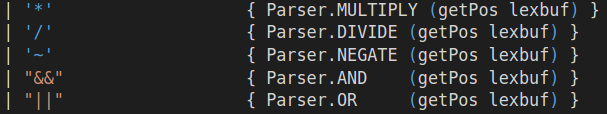
\includegraphics[width=\linewidth]{Materials/Lexer/Lexer}

        \section{Parser}
Once the lexer has recognized input, the parser is in charge of handling said input. For example, if the lexer recognizes an \textit{or}-expression, the parser must determine if the semantics are in order - for example if the \textit{or}-operator is used, it must check if the operator is used on two expressions in a proper maner. If not, the parser must recognize this and a parsing-error will occur. Returning to the \textit{or}-operator, it only makes sense if the \textit{or}-keyword is sandwiched between two expressions or else the use of the \textit{or}-operator doesn't fit its formal definition. The parser checks if this is the case, and if so, calls upon the typechecker to ensure the types of the expressions are in order. The check, which the parser makes, looks like this in our implementation:\\
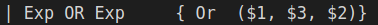
\includegraphics[width=\linewidth]{Materials/Parser/Or}\\
This implementation ensures that only the \textit{or}-operator when sandwiched between two expressions is accepted, or else an error will be raised. 

        \section{Typechecker}
An fs file \textit{TypeChecker.fs} has been implemented, the purpose of which is to ensure that the types, on which arithmetic operators (\textit{plus,minus,etc.}), logical operators (\textit{and,or}) and others, match the given operator.
For example, if we want to implement the \textit{or}-operator, we need to ensure that the operator will only be aplied on boolean values, as any other values don't make sense given the specification of the \textit{or}-operator.\\
The implementation of the typechecker for the \textit{or}-operator, can be seen here: \\
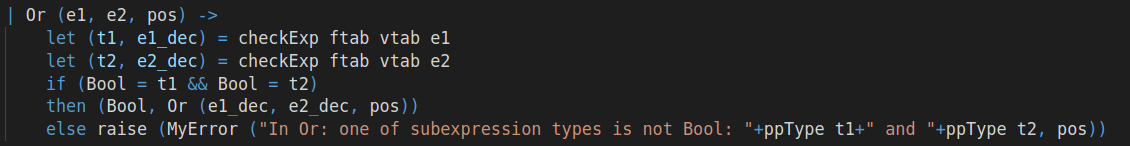
\includegraphics[width=\linewidth]{Materials/TypeChecker/Or}\\
Focusing on the \textit{or}-operator (since other operators are implemented in largely the same way), the typechecking works as follows:\\
First, we call the checkExp function and match with the \textit{Or}-keyword and parse it the two expressions no which we operator and the position.
Afterwards, we determine the type of our expressions by calling the checkExp function whilst supplying it our Function-table and Value-table.\\
Next, we check that both types match (i.e are boolean values). If so, we run theimplemented \textit{or}-function as found in \textit{codeGen.fs} on our expressions, which we now know to be of the type bool. If the \textit{or}-operator is not called on bools, we raise an error stating that at least one of the expressions is of the wrong type.\\
The typechecker works the same for all other operators, except possibly checking on other types like Ints for an arithmetic operator. 

	\section{CodeGen}
\subsection{Filter}
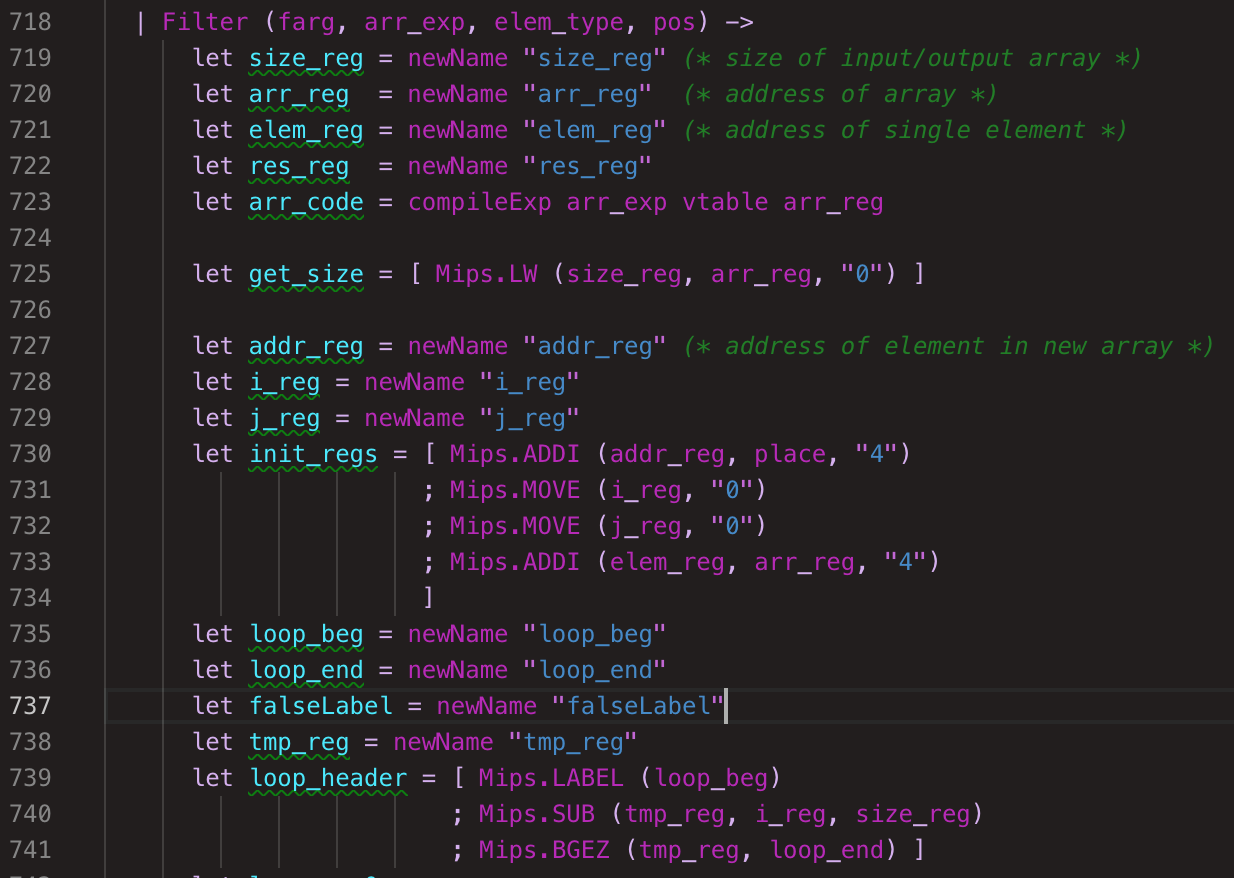
\includegraphics[width=\linewidth]{Materials/CodeGen/filterIntro}
Filter is implemented much like 'map'. To implement filter we first create a new array of the same size as the input array. We also create some new registers to keep track of the memory locations of the elements in the new array (\textit{addr\_reg}) and the input array (\textit{elem\_reg}). Lastly we create a register (\textit{j\_reg}) to count how many elements we have added to the new array.\\
The idea is we create a loop where we apply the input function on the first element of the input array, and if the output is \textit{true} we then add it to the new array, we add to the registers working as pointers to the elements in the array such that we move to the next entry in the arrays and lastly we add one to our counter register \textit{j\_reg}. If the output is \textit{false}, we only add to the \textit{elem\_reg} and then begin the loop anew on the next element of the input array.\\
We do this by loading the value of the input array into \textit{res\_reg} and apply the input function using the helper function \textit{applyFunArg} on lines 742-747.
 
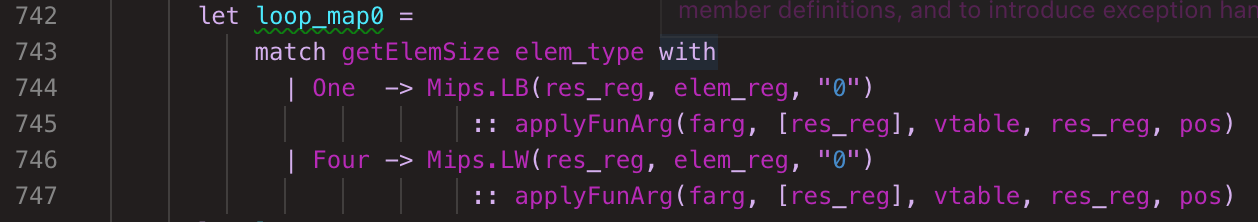
\includegraphics[width=\linewidth]{Materials/CodeGen/filter1}
We now have either '1' or '0' (true, false) in \textit{res\_reg}. We now load the value of \textit{elem\_reg} into a temporary register for use if the result is true. Then we add to \textit{elem\_reg} to have it point to the next entry of the input array. We now do a conditional branching. If the value of \textit{res\_reg} is true, we fall through, else we jump. In the case the result is \textit{true}, we save the value in \textit{tmp\_reg} in \textit{addr\_reg}, we add to \textit{addr\_reg} such that it points to the next entry of the array and we add 1 to \textit{j\_reg}. Then we meet the point where we would jump to if the result had been false (line 762), and the loop begins anew. All of this is done on lines 748-765. When the loop terminates after having iterated over all entries in the input array, we then shrink the size of our new array to its actual size using \textit{j\_reg} on line 766.

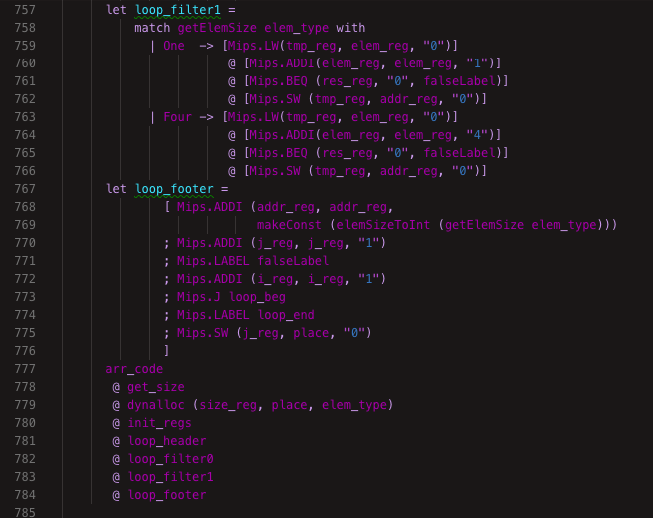
\includegraphics[width=\linewidth]{Materials/CodeGen/filter2}
\subsection{Replicate}
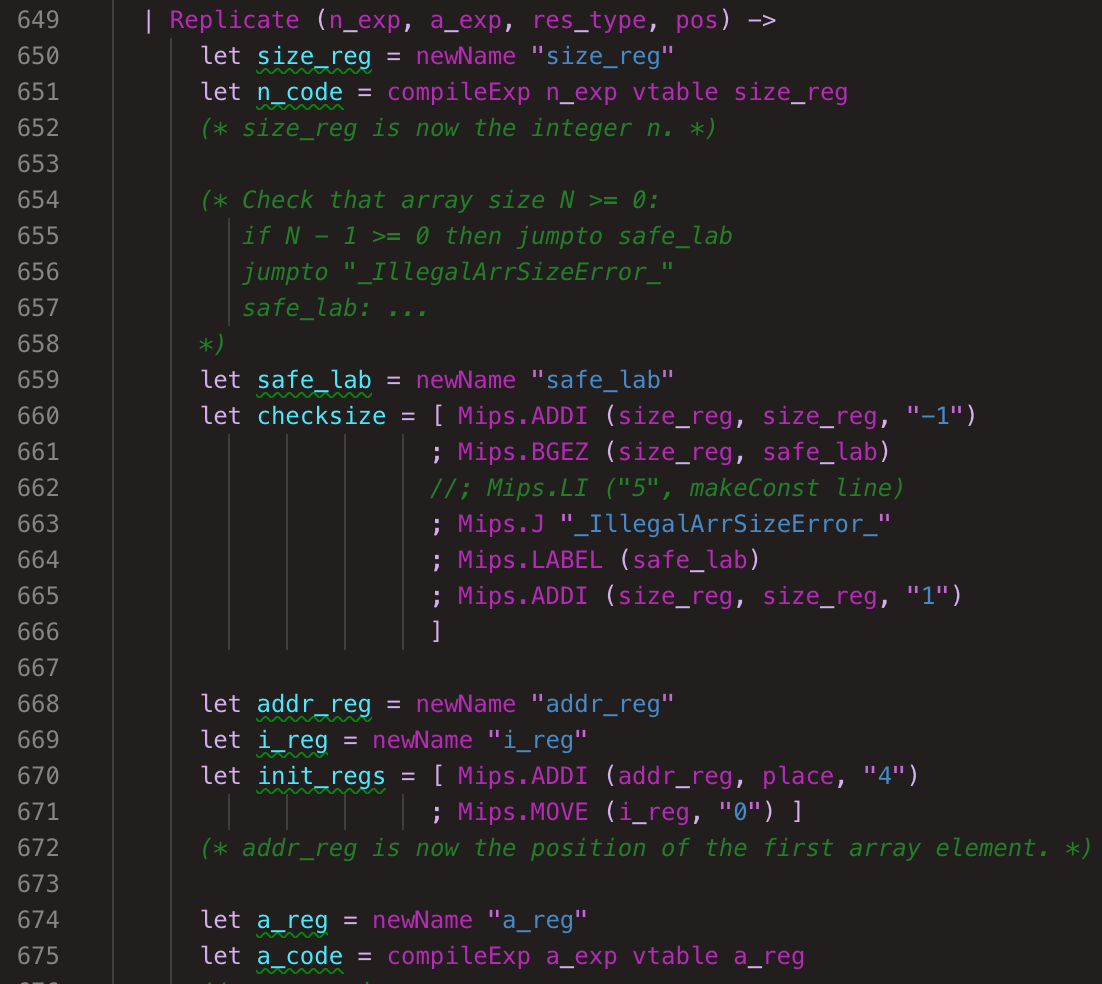
\includegraphics[width=\linewidth]{Materials/CodeGen/ReplicateIntro}
To implement replicate we first check if the given '\textit{n expression}' is greater than zero, and then we create a new array of size \textit{n} (lines 650-666). Then we create a register \textit{addr\_reg} which points to the first entry in the new array and we create another register \textit{a\_reg} which contains our given input which we want to replicate.\\
The idea is we create a loop and in each iteration we put the value of \textit{a\_reg} into the new array.\\
First we save the value of \textit{a\_reg} in \textit{addr\_reg} such that the entry in the new array which \textit{addr\_reg} points to now contains the replicated value. Then we add to \textit{addr\_reg} so it points to the next entry and we update the loop counter \textit{i\_reg} and start the loop anew. All of this is done on lines 680-693.\\
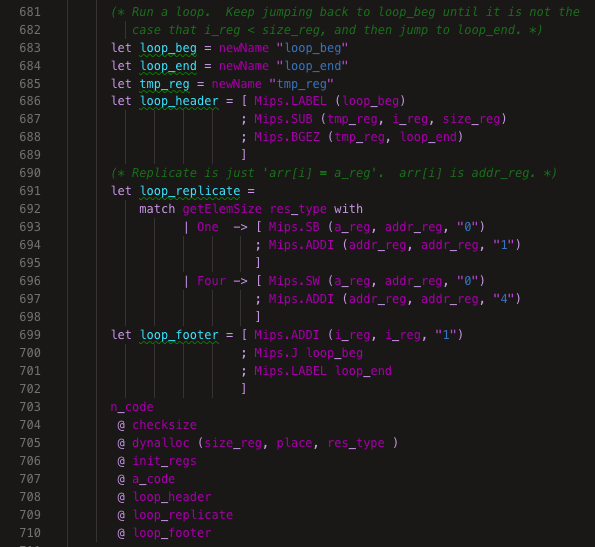
\includegraphics[width=\linewidth]{Materials/CodeGen/Replicate1}

\subsection{Scan}
The idea is we create a register to hold the accumulated value. Then we create a loop in where we apply the supplied function on the value in the accumulated register and the element in the input array and we save the value in the accumulated register. Then we save the value in the accumulated register in the new array and we begin the loop anew.
\end{document}
